\documentclass[12pt,a4paper]{article}

% =========================
% Packages
% =========================
\usepackage[utf8]{inputenc}
\usepackage[T1]{fontenc}
\usepackage[english]{babel}
\usepackage{graphicx}
\usepackage{geometry}
\usepackage{hyperref}
\usepackage{enumitem}
\usepackage{placeins}

\geometry{
    margin=2.5cm
}
\raggedbottom

\hypersetup{
    colorlinks=true,
    linkcolor=blue,
    urlcolor=blue
}

\graphicspath{{../design/}{assets/}}

% =========================
% Metadata
% =========================
\title{\textbf{SAP Report}\\
\large Design and Implementation of a Microservices-Based Application}
\author{Rosario Zaccone}
\date{June 2026}

\newcommand{\reportversion}{v0.1.26}
\newcommand{\reportlastmodified}{2026-07-26}

\begin{document}

\maketitle

\begin{center}
    \textbf{Version:} \reportversion\\
    \textbf{Last Modified:} \reportlastmodified\\
    \textbf{GitHub Repository:} \url{https://github.com/rosario-zaccone/rione}
\end{center}

\tableofcontents
\newpage

% =========================
% 1. Application Description
% =========================
\section{Application Description}

Rione is a social network centred on small local communities. Its purpose is to support interaction among people who live in the same neighbourhood, limiting the social space to nearby residents rather than creating a broad and generic online network. The platform is based on the idea that digital communication can become more useful and meaningful when it is connected to the places in which people live their everyday lives.

The core principle of the project is neighbourhood-based interaction. Users can see and interact only with other users who belong to the same neighbourhood. For example, in a city such as Bologna, neighbourhoods may include Navile, Saragozza, San Vitale, Savena, and others. A user who belongs to Navile should interact only with other users from Navile, while users from different neighbourhoods remain outside that local social space. This constraint gives the platform a clear community boundary and distinguishes it from traditional social networks, where interactions are often global, anonymous, or weakly connected to real-life contexts.

The motivation behind Rione is to create a more local and purposeful form of online participation. By focusing on neighbourhood communities, the platform aims to strengthen relationships among nearby residents, encourage participation in local community life, and make online exchanges more relevant to practical daily needs. A local social network can help people share information, ask for help, discuss neighbourhood issues, organize small events, and become more aware of what happens around them.

Another important motivation is trust. Interactions among people who share the same local environment can be more concrete than interactions in large-scale social networks. The neighbourhood boundary encourages users to perceive other participants not as distant strangers, but as members of the same local community. This can increase the perceived value of contributions and support more responsible communication.

The platform also introduces deliberate constraints to promote more thoughtful participation. For instance, posts and comments may require a minimum length, encouraging users to write meaningful contributions instead of very short or superficial messages. These constraints are intended to increase attention, reduce low-effort interactions, and improve the quality of discussions. In this sense, Rione is designed not only as a communication tool, but also as a way to encourage more careful, relevant, and community-oriented digital participation.

% =========================
% 2. Technological Choices
% =========================
\section{Technological Choices}

This section describes the main technologies and development tools used in the project. The stack was chosen to support the main goals of the assignment: a microservices architecture, explicit domain modeling, testable business logic, observable runtime behavior, and a local environment that can be started and inspected easily.

\subsection{Technologies Used}

The project is implemented as a Maven multi-module application. This structure keeps all services in one repository while preserving separate modules, dependencies, tests, and build targets. It is useful for an academic project because the whole system can be built with one command, but each service can still be developed and verified independently.

The backend uses Java and Spring Boot because they provide a mature ecosystem for REST APIs, validation, security, persistence, testing, and observability. Docker Compose is used for local execution because the system depends on several runtime components, including databases, Kafka, Prometheus, Grafana, and pgAdmin. Running them through Compose makes the deployment reproducible and keeps the local environment close to the architecture described in Figure~\ref{fig:deployment-architecture}.

\begin{itemize}
    \item \textbf{Java 21}: used as the main backend language. It was selected because it is strongly typed, works well with DDD-style models, and integrates naturally with Spring Boot.
    \item \textbf{Spring Boot 4.1.0}: used as the base framework for the backend services. It provides the runtime conventions, dependency injection, configuration model, actuator endpoints, and testing support needed by each service.
    \item \textbf{Spring Web MVC}: used to expose REST APIs. Controllers are kept in the infrastructure layer and translate HTTP requests into application use case calls.
    \item \textbf{Spring Data JPA}: used in persistence adapters for relational data. It keeps database access outside the domain model and allows repositories to implement output ports.
    \item \textbf{PostgreSQL}: used as the relational database for services that own persistent state. Each service has its own schema or database boundary, which supports the database-per-service approach.
    \item \textbf{Apache Kafka}: used for asynchronous communication when one service must react to another service's event without blocking the original workflow. This is especially important for notifications.
    \item \textbf{Spring Security}: used for JWT-based user authentication, role-based authorization, and service-to-service protection for internal APIs.
    \item \textbf{Springdoc OpenAPI}: used to publish API documentation from the implemented controllers. The generated contracts are also used to create the API diagrams shown later in the report.
    \item \textbf{React and Vite}: used to build a lightweight frontend that exercises the application through the API Gateway. It was mainly used for manual end-to-end testing and demonstration.
    \item \textbf{Docker and Docker Compose}: used to package and run services, databases, Kafka, Prometheus, Grafana, and pgAdmin in a reproducible local environment.
    \item \textbf{Prometheus and Grafana}: used to collect and visualize technical and business metrics, making service behavior visible during local execution.
    \item \textbf{Maven}: used for dependency management, module builds, and test execution. The Maven reactor makes it possible to verify a single service or the whole system.
    \item \textbf{GitHub and GitHub Actions}: used for version control and continuous integration, so tests and build checks run automatically on relevant branches and pull requests.
\end{itemize}

% =========================
% 3. Testing Architecture
% =========================
\section{Testing Architecture}

The testing strategy is organized around Test-Driven Development and layered verification. Business rules are first expressed in requirements documents and then mapped to executable tests. This was done to keep tests connected to the documented behavior instead of treating them as an afterthought written only after the code was complete.

The project follows the idea of the testing pyramid. At the base of the pyramid there are many fast unit tests, because they are cheap to execute and give quick feedback on domain and application logic. In the middle there are integration tests, which are fewer because they involve frameworks, adapters, persistence, security, messaging, or HTTP boundaries. At the top there are higher-level acceptance tests, which are more expensive but validate business behavior from the user's point of view. Architecture tests are used as an additional technical guardrail to verify that the intended code structure is preserved.

Each main business service follows the same testing structure under \texttt{src/test}. The project separates acceptance tests, architecture tests, integration tests, and unit tests. This separation keeps each test focused on a specific risk: business correctness, architectural conformance, adapter behavior, or isolated domain and application logic.

The test suite is executed with Maven. During continuous integration, GitHub Actions runs \texttt{verify} on each service and then on the full Maven reactor. This means that a change is validated both in its own module and in the context of the whole project. The approach is intentionally practical: fast tests give immediate feedback while integration and acceptance tests protect the most important service boundaries.

\subsection{Types of Tests}

The project uses four main test layers.

\begin{itemize}
    \item \textbf{Unit Tests}: unit tests verify small units of behavior in isolation. They are placed at the base of the testing pyramid because they are fast, deterministic, and numerous. In this project, they are implemented with JUnit and Mockito and focus on domain models, value objects, and application services. Examples include tests for user value objects such as biography, birth date, and password, and service tests for user, social, post, and notification application logic.
    \item \textbf{Integration Tests}: integration tests verify that multiple components work correctly together across technical boundaries. They occupy the middle level of the testing pyramid because they are slower than unit tests but provide stronger confidence in framework and adapter behavior. In this project, they are implemented with JUnit and Spring testing support and verify REST controllers, security configuration, JWT handling, JPA repositories, Kafka adapters, metrics configuration, and schema migration behavior.
    \item \textbf{Architecture Tests}: architecture tests verify structural constraints rather than business behavior. They check that the implementation respects the intended separation between domain, application ports, application services, and infrastructure adapters. In this project, they are implemented with ArchUnit and act as automated guardrails against accidental dependency violations.
    \item \textbf{Acceptance Tests}: acceptance tests verify the system behavior expected by the requirements. They are placed at the top of the testing pyramid because they validate broader business scenarios. In this project, they are implemented with Gherkin, Cucumber, and JUnit, and they are explicitly modeled on the documented business rules. Feature files use stable rule identifiers such as \texttt{USR-BR-001}, \texttt{SOC-BR-001}, \texttt{PST-BR-006}, and \texttt{NOT-BR-001}, so each acceptance scenario can be traced back to a specific business rule.
\end{itemize}

This combination gives the project broad coverage without relying on a single kind of test. Unit tests keep domain logic fast to verify, integration tests validate the collaboration with frameworks and adapters, architecture tests prevent accidental dependency violations, and acceptance tests protect the business requirements defined in the requirements documentation.

\subsection{CI/CD Pipeline}

The repository uses GitHub Actions to automatically verify the project. The current pipeline is focused on continuous integration: it checks that the services compile and that their automated tests pass before changes are considered safe to merge. This is useful in a multi-service project because a change in one module can still break another module through shared contracts, build configuration, or service integration code.

\begin{itemize}
    \item The workflow runs on pushes to \texttt{feature/**} branches and to \texttt{main}.
    \item The workflow also runs on pull requests targeting \texttt{main}.
    \item A matrix job verifies the main backend services independently: User Service, Post Service, Social Service, and Notification Service.
    \item Each service job uses Java 21 and executes \texttt{./mvnw -B -pl <module> verify}.
    \item After the service-level jobs, a full Maven reactor verification is executed with \texttt{./mvnw -B verify}.
    \item Maven dependency caching is enabled through the Java setup action to reduce build time.
\end{itemize}

This pipeline supports a test-first and regression-aware workflow. The goal is to detect broken business rules, architectural violations, integration problems, or compilation errors before they reach the main branch.

% =========================
% 4. Domain-Driven Design Approach
% =========================
\section{Domain-Driven Design Approach}
The project uses Domain-Driven Design as required by the exam assignment. DDD was adopted because Rione is not only a CRUD application: it has rules about neighbourhood membership, visibility, social relationships, blocking, post privacy, reactions, comments, and notifications. These rules are easier to understand and protect when the code uses the same concepts as the domain.

In practice, DDD was used to keep business decisions separate from technical details such as REST controllers, persistence, messaging, and infrastructure configuration. The domain model captures the core rules, while adapters translate between the model and external mechanisms.

\subsection{Strategic Design}

Strategic design was used before implementation to understand the problem space and choose service boundaries. The domain was divided into clear business areas, each with its own model, responsibilities, and language. This avoided a single shared model that would mix identity, relationships, posts, and notifications into one large and fragile component.

\subsubsection{Bounded Contexts}

The analysis started from the overall domain and from conceptual sketches of the main domain components. From this view, four bounded contexts were identified: User, Social, Post, and Notification. Each bounded context owns a specific part of the domain: the User context manages user identity and profile information, the Social context manages neighbourhood membership and relationships, the Post context manages publications and interactions with content, and the Notification context manages the delivery of relevant events to users.

These contexts also correspond to the main business microservices of the system. This mapping is deliberate: each service owns a coherent set of rules and can evolve its model without forcing other services to share its internal classes or database tables.

\subsubsection{Context Map}

Identifying bounded contexts is not enough on its own: strategic design also requires defining how these contexts relate to each other, since the boundaries do not by themselves describe the level of coupling between services. The relationship between the User context and both the Social and Post contexts follows an Anticorruption Layer pattern. The Social and Post services depend on user data, but neither adopts the User context's model directly: each defines its own outbound port in its own ubiquitous language (for example, \texttt{UserProfile} in the Social Service) and a dedicated proxy adapter that translates the User Service response into that local vocabulary before it reaches the domain. The same pattern applies between the Social and Post contexts, where the Post Service resolves relationship visibility (same neighbourhood, active neighbourship, blocking) through a proxy that translates the Social Service response into its own \texttt{RelationshipVisibility} value object. In both cases the downstream service acts as the customer and the upstream service as the supplier, but the translation guarantees that no context is forced to conform to another context's internal model.

The relationship between the Social and Notification contexts is different: it is asynchronous and event-based rather than a direct request-response call. The Social Service publishes domain events as JSON messages to a Kafka topic without knowing which services consume them; the Notification Service listens independently and reacts only to the events it needs. The event schema acts as a Published Language shared between the two contexts, and the stable topic and message contract represent an Open Host Service exposed by the Social context. This keeps the two services decoupled in time and avoids a synchronous dependency for a concern, notification delivery, that does not need to block the use case that originates it.

No Shared Kernel exists between the bounded contexts: the only shared module, \texttt{common}, contains DDD marker annotations rather than domain model or business logic. As a result, every cross-context dependency is either an explicit Anticorruption Layer over a synchronous call or a Published Language over an asynchronous event, and no context depends on another context's internal classes, database, or domain types.

The full context map, including the per-relationship rationale and the concrete ports and adapters involved, is documented in:

\begin{itemize}
    \item \path{docs/design/context_map.md}
\end{itemize}

\subsubsection{Ubiquitous Language}

Each bounded context has its own ubiquitous language, documented in the glossary files. The glossary defines the main terms used in requirements, code, tests, and diagrams, so that the same concept is described consistently across the project. This is especially important because similar words can have different meanings in different contexts: for example, a user profile belongs to the User context, while neighbourhood membership belongs to the Social context.

\begin{itemize}
    \item \path{docs/requirements/user/ubi_language.md}
    \item \path{docs/requirements/social/ubi_language.md}
    \item \path{docs/requirements/post/ubi_language.md}
    \item \path{docs/requirements/notification/ubi_language.md}
\end{itemize}

\subsection{Tactical Design}

For each bounded context, a UML domain model was designed before implementation and is presented later in the report. These diagrams identify the main aggregates, entities, value objects, and relationships used by the services. They provide a bridge between the requirements documentation and the code, making the domain structure inspectable before reading implementation details.

In the implementation, tactical DDD patterns are used to make the model explicit. Entities represent domain concepts with identity, value objects represent immutable concepts defined by their attributes, and aggregate roots protect consistency boundaries. The code also uses project-specific DDD annotations, such as \texttt{DDDEntity}, \texttt{DDDValueObject}, and \texttt{DDDAggregateRoot}, to make these roles visible and easier to verify.

Value objects are also used to encapsulate validation rules for meaningful attributes. Instead of passing raw strings, numbers, or identifiers through the system, concepts such as e-mail addresses, biographies, names, identifiers, post content, and places are created through dedicated types that validate their own state. This choice keeps invalid values from entering the domain model, avoids duplicating the same checks in controllers or services, and makes the code more expressive because the type itself communicates the meaning and constraints of the value.

Aggregate roots are responsible for the lifecycle of the entities connected to them. External code interacts with the aggregate through the root, while the root creates, updates, removes, or protects internal entities according to the aggregate invariants. For example, comments and reactions are managed through the Post aggregate rather than being modified independently. This keeps related state changes consistent and prevents application services or adapters from bypassing domain rules.

The same idea is reflected in the application structure. Domain rules are kept in the domain model, application services coordinate use cases, and infrastructure adapters handle external concerns such as HTTP, persistence, and messaging. This keeps the core model independent from technical mechanisms and supports the hexagonal organization used by the services.

% =========================
% 5. Requirements
% =========================
\section{Requirements}

Requirements were written before implementation and were used as the main input for design, testing, and AI-assisted coding. This made the work traceable: user stories describe the expected value, SRS tables turn that value into system responsibilities, and business rules define the constraints that tests and domain logic must enforce.

The requirements documentation is stored in the following folders:

\begin{itemize}
    \item \path{docs/requirements/api-gateway/}
    \item \path{docs/requirements/user/}
    \item \path{docs/requirements/social/}
    \item \path{docs/requirements/post/}
    \item \path{docs/requirements/notification/}
\end{itemize}

\subsection{User Stories}

User stories are short requirement descriptions written from the perspective of an actor. They describe who needs a capability, what they want to do, and why the capability has value. In this project they were used to keep implementation decisions connected to actual user goals, instead of starting directly from controllers or database tables.

The user stories are stored in:

\begin{itemize}
    \item \path{docs/requirements/api-gateway/user_stories.md}
    \item \path{docs/requirements/user/user_stories.md}
    \item \path{docs/requirements/social/user_stories.md}
    \item \path{docs/requirements/post/user_stories.md}
    \item \path{docs/requirements/notification/user_stories.md}
\end{itemize}

\subsection{Requirements Tables}

Requirement tables translate user stories into structured system responsibilities. They assign stable identifiers to functional requirements, business rules, and non-functional requirements. These identifiers are useful because they can be referenced by tests, implementation tasks, and report sections without relying on vague descriptions.

The requirement tables are stored in the Software Requirements Specification files:

\begin{itemize}
    \item \path{docs/requirements/api-gateway/srs.md}
    \item \path{docs/requirements/user/srs.md}
    \item \path{docs/requirements/social/srs.md}
    \item \path{docs/requirements/post/srs.md}
    \item \path{docs/requirements/notification/srs.md}
\end{itemize}

\subsection{Business Rules}

Business rules are domain constraints that must remain true regardless of the technical interface used to execute an operation. They define when an operation is valid, what must be rejected, and which side effects are allowed. For this reason, they belong close to the domain model and are also reflected in acceptance tests.

The business rules are documented in the same requirements folders as the user stories and SRS files:

\begin{itemize}
    \item \path{docs/requirements/api-gateway/}
    \item \path{docs/requirements/user/}
    \item \path{docs/requirements/social/}
    \item \path{docs/requirements/post/}
    \item \path{docs/requirements/notification/}
\end{itemize}

\subsection{Quality Attribute Scenarios}

The SRS tables capture non-functional requirements as short statements, but a statement such as ``the system must be scalable'' is not by itself testable. Quality Attribute Scenarios (QAS) make each attribute concrete by fixing six fields: source of stimulus, stimulus, environment, artifact, response, and response measure. Unlike the rest of the requirements documentation, these scenarios were written after the architecture was already implemented rather than before, since they were not part of the original requirements pass. For this reason, each scenario is paired with evidence already present in the codebase (a test, a configuration, or a metric) that lets the response measure be checked directly instead of only asserted.

Six scenarios are documented, one per attribute: Availability (the api-gateway's circuit breaker isolating a failing downstream service), Performance (read latency on the Post Service, currently measured as an average rather than a percentile), Modifiability (a domain rule change staying confined to \texttt{domain}/\texttt{application}, checked by ArchUnit), Testability (a business rule change caught by the CI suite before merge), Security (a request without a valid JWT being rejected before reaching business logic), and Scalability (a single microservice being redeployed or scaled independently of the others).

The full scenarios are documented in \path{docs/design/quality_attribute_scenarios.md}.

% =========================
% 6. Application Architecture
% =========================
\section{Implementation and Deployment Architecture}

The system is implemented as a microservices architecture. This choice was made because the domain naturally separates into areas with different responsibilities: user identity, social relationships, posts, and notifications. Each main bounded context identified during the DDD analysis corresponds to a business microservice: User Service, Social Service, Post Service, and Notification Service. This decomposition keeps each service responsible for a coherent part of the domain and allows each model to evolve without forcing all services to share the same internal representation.

Additional services and infrastructure components were added to support cross-cutting concerns. The API Gateway exposes a single entry point for the frontend and routes requests to the backend services, so clients do not need to know the internal service topology. PostgreSQL databases provide persistence for services that own durable state, while Kafka is used as the event broker for asynchronous communication. Monitoring components, such as Prometheus and Grafana, run with the application to make service health and runtime metrics visible.

Synchronous communication between microservices is implemented through REST APIs. It is used only when a service needs immediate information from another service to complete a use case. To keep this dependency explicit and isolated, services use proxy clients in the infrastructure layer. For example, the Social Service may need user information that goes beyond the user identifier; through a User Service proxy, it can retrieve the required user details without directly accessing the User Service database or sharing its internal domain model. The resulting deployment view is shown in Figure~\ref{fig:deployment-architecture}.

\begin{figure}[htbp]
    \centering
    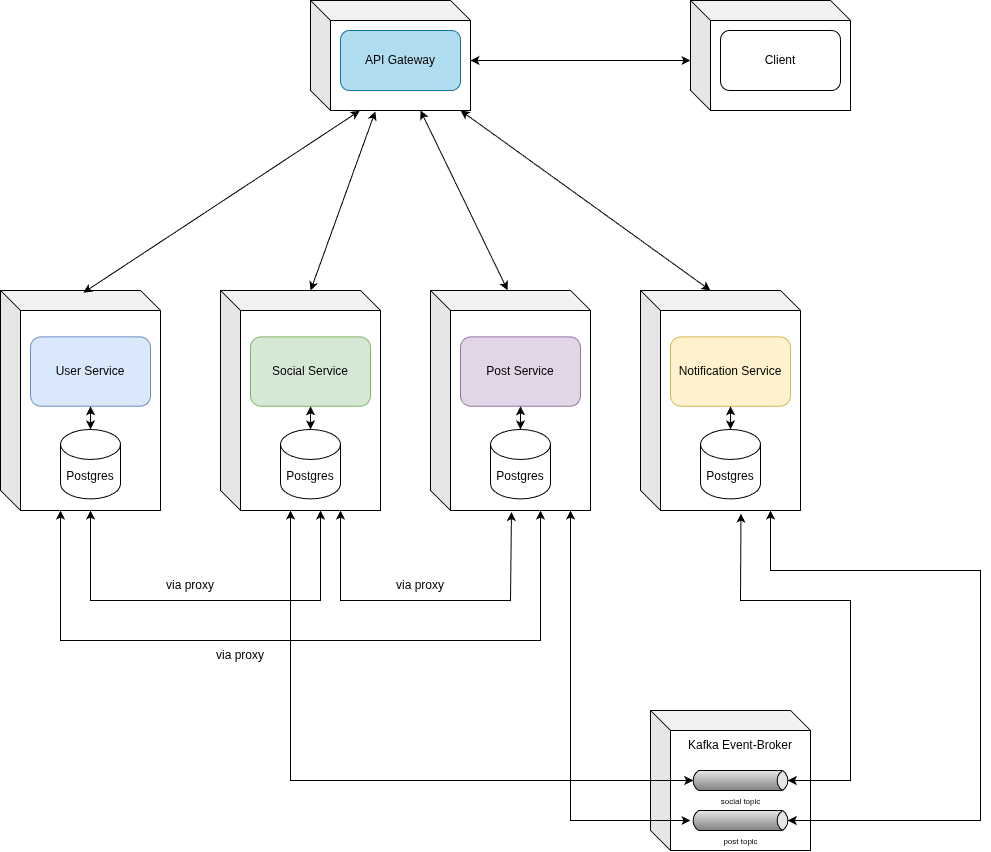
\includegraphics[width=0.95\textwidth]{deployment_architecture.png}
    \caption{Deployment architecture of the Rione system.}
    \label{fig:deployment-architecture}
\end{figure}

\subsection{Clean and Hexagonal Service Structure}

The business microservices follow a clean and hexagonal organization. This pattern was used to protect the domain model from framework and infrastructure details. Each service is divided into domain, application, and infrastructure layers. The domain layer contains the core business model and rules; the application layer coordinates use cases and defines ports; the infrastructure layer contains adapters for REST APIs, persistence, messaging, configuration, and external integrations.

This structure keeps dependencies directed toward the inner layers. Controllers, repositories, Kafka consumers, REST proxy clients, and other technical details depend on the application and domain model, while the domain model does not depend on Spring, databases, HTTP, or Kafka. This makes the business logic easier to test and reduces the impact of changing an external technology. The dependency direction is summarized in Figure~\ref{fig:clean-architecture}.

\begin{figure}[htbp]
    \centering
    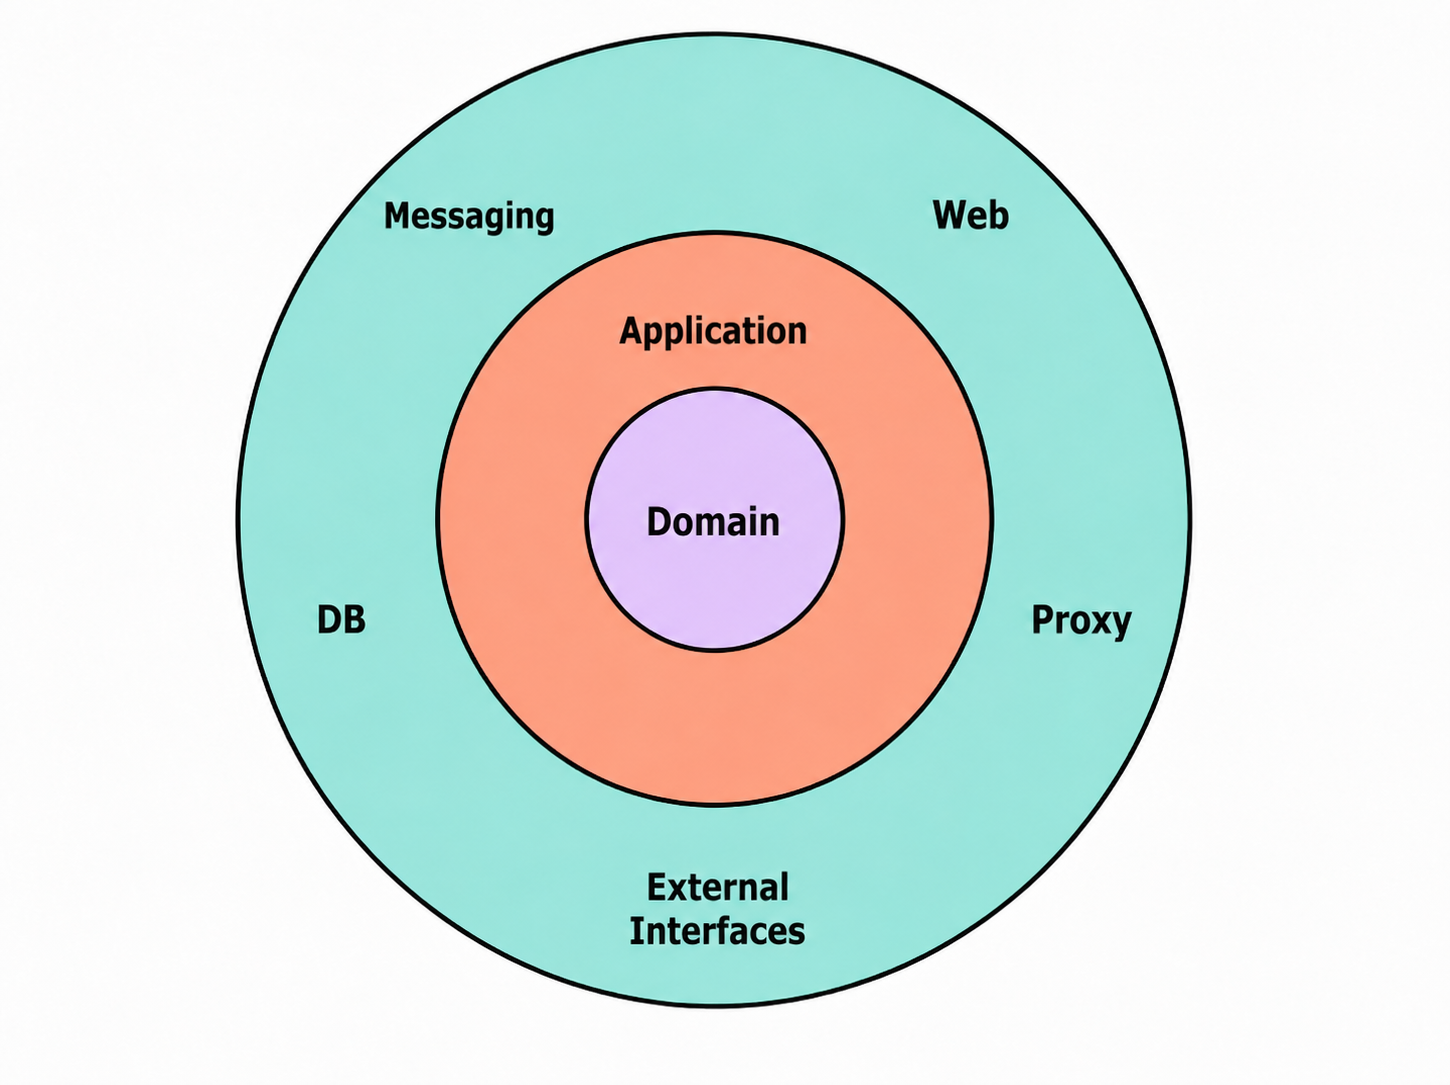
\includegraphics[width=0.75\textwidth]{clean.png}
    \caption{Clean Architecture dependency direction adapted to the Rione service structure.}
    \label{fig:clean-architecture}
\end{figure}

\subsection{Event-Driven Communication}

An event-driven approach is used where asynchronous communication is more appropriate than direct synchronous calls. This is especially useful for notifications, because a user action such as sending a neighbour request or commenting on a post should not fail only because notification processing is temporarily unavailable. For this reason, the Notification Service reacts to events produced by other services instead of being called directly by each workflow that may generate a notification.

Kafka acts as the event broker. The Post Service and Social Service publish events on Kafka topics when relevant domain actions occur, and the Notification Service consumes those events to create notifications. This design reduces coupling between the services that produce business events and the service that handles notifications. It also makes the notification workflow more scalable, because event producers do not need to wait for notification processing to complete before finishing their own use cases.

\subsection{Application Security}

Security is managed with Spring Security and JWT-based stateless authentication. This was chosen because the system is distributed: relying on server-side HTTP sessions would make authentication harder to share across services. The User Service is responsible for user registration and login: credentials are validated there, passwords are stored as hashes rather than plain text, and a JWT is returned after a successful login. Clients then send the token in the \texttt{Authorization: Bearer <token>} header when calling protected APIs. Each backend service validates the token before executing protected operations.

The security configuration explicitly separates public, authenticated, administrative, and internal endpoints. Public routes include login, registration, selected read-only resources, health checks, Prometheus scraping, and OpenAPI documentation. Business operations require an authenticated user, and administrative operations such as city management are protected with an admin role. Controllers do not parse tokens directly; instead, JWT validation is handled by a security filter, and controllers retrieve the current user from the Spring Security context. This keeps authentication concerns outside the domain and application logic.

Service-to-service communication is protected with dedicated service tokens. Internal APIs are exposed under \texttt{/internal/**} and require \texttt{ROLE\_SERVICE}; they are intended for backend services, not for frontend clients. For example, the Social Service and Post Service can call the User Service through proxy adapters to retrieve only the minimal user information needed by their use cases. These calls use short-lived service JWTs signed with a separate service secret and validated with service-specific claims such as service identity and target audience. This prevents services from reusing user tokens or accessing another service database directly, while still allowing the system to enforce cross-service rules such as neighbourhood visibility and post privacy.

% =========================
% 7. Main Microservices
% =========================
\section{Main Microservices}

This section presents the main microservices of the system. Each business service is described through its API contract, domain model, and component-and-connector view. The API diagrams are derived from the OpenAPI specifications in \path{docs/openapi/}, while the domain diagrams are generated from the PlantUML models in \path{docs/design/}.

\subsection{API Gateway}

The API Gateway is the public entry point of the backend. It was introduced to give clients one stable HTTP boundary instead of exposing each internal service directly. The gateway exposes the routes consumed by the frontend and forwards requests to the internal services, keeping clients independent from the internal service topology. It does not own a domain model; its responsibility is API composition, routing, cross-origin access, and boundary-level access to backend capabilities. Its public API surface is illustrated in Figure~\ref{fig:api-gateway-openapi}.

\begin{figure}[htbp]
    \centering
    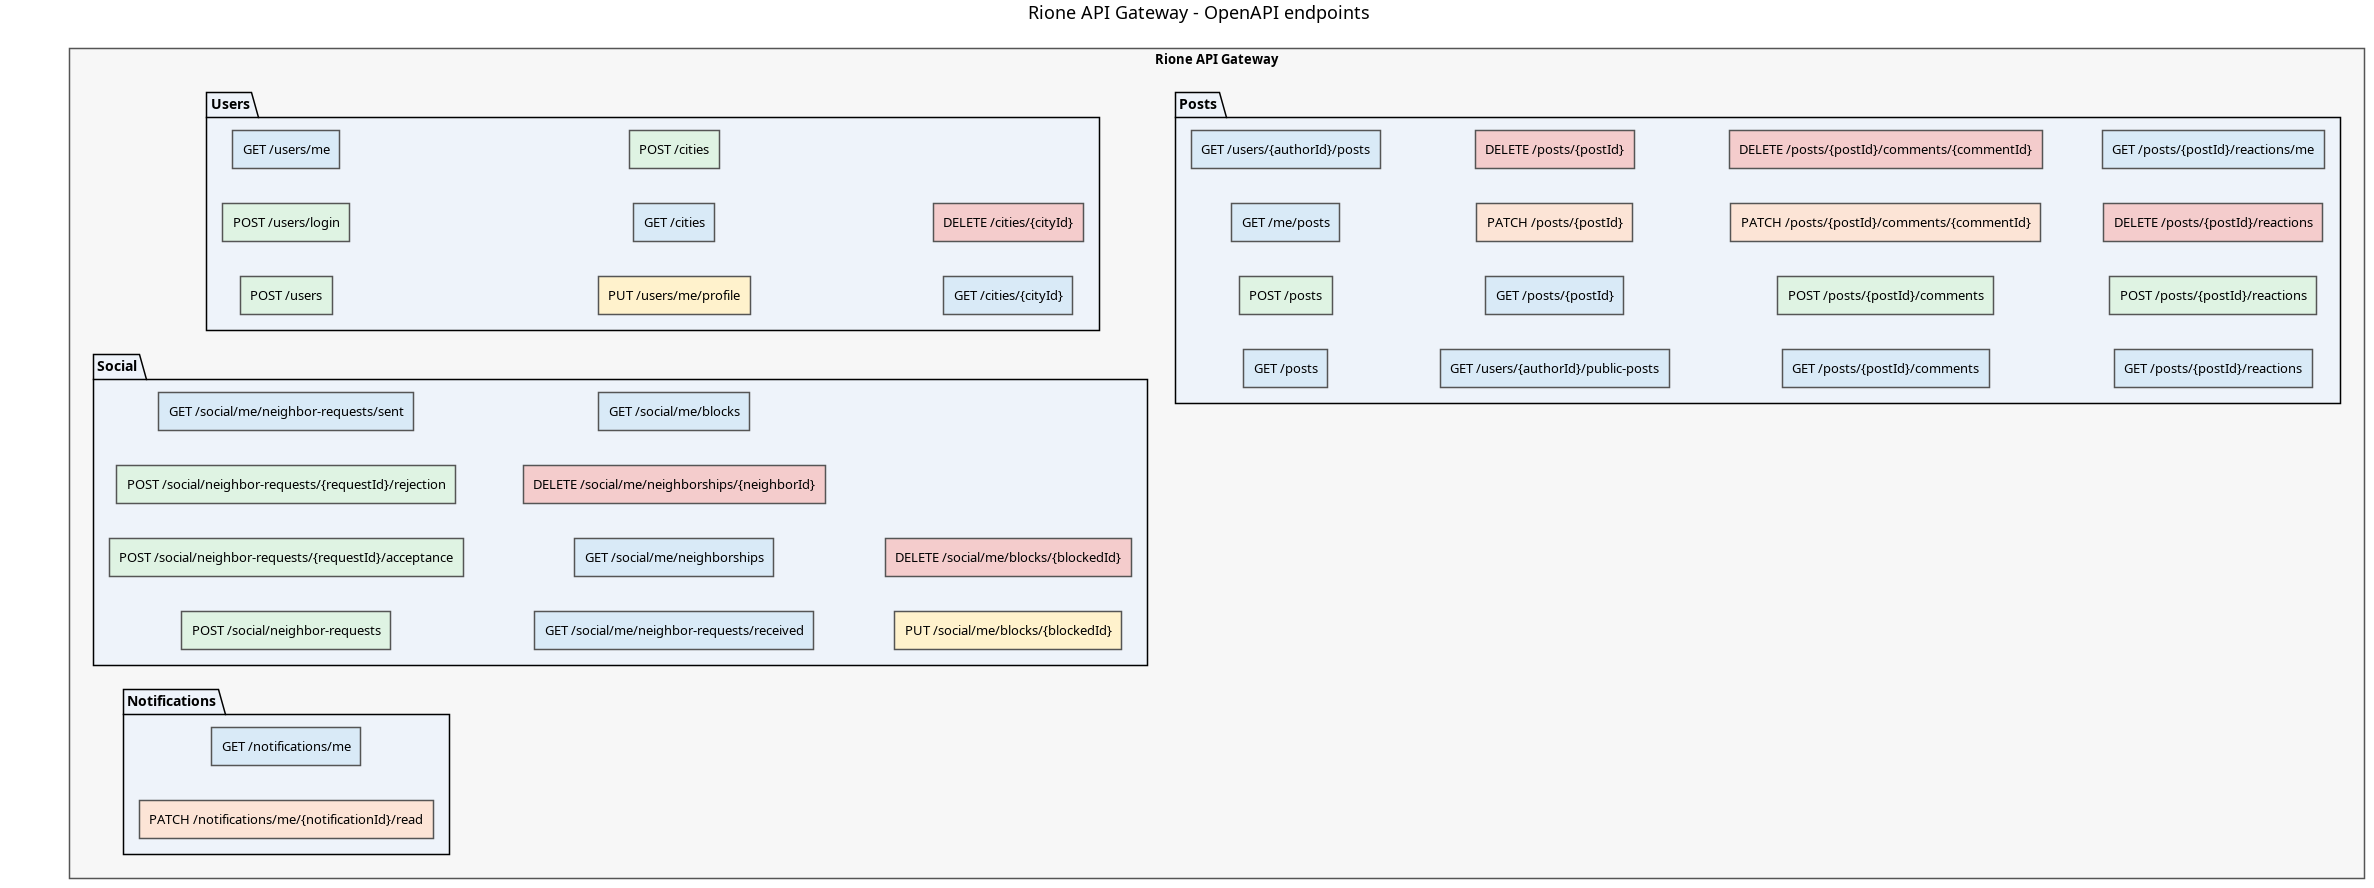
\includegraphics[width=0.95\textwidth]{generated/api-gateway_api.png}
    \caption{API Gateway OpenAPI diagram.}
    \label{fig:api-gateway-openapi}
\end{figure}

\FloatBarrier

\subsection{User Service}

The User Service manages identity and profile-related information. It owns this data because authentication, profile information, and neighbourhood membership must have one authoritative source. Its domain model includes users, cities, neighbourhoods, and value objects such as user identifiers, names, mail addresses, and biographies. The service also exposes internal endpoints used by other services when they need user-related information without accessing the User Service database directly. Its API contract is shown in Figure~\ref{fig:user-service-openapi}, its domain model in Figure~\ref{fig:user-service-domain}, and its component-and-connector view in Figure~\ref{fig:user-service-cc}.

\begin{figure}[htbp]
    \centering
    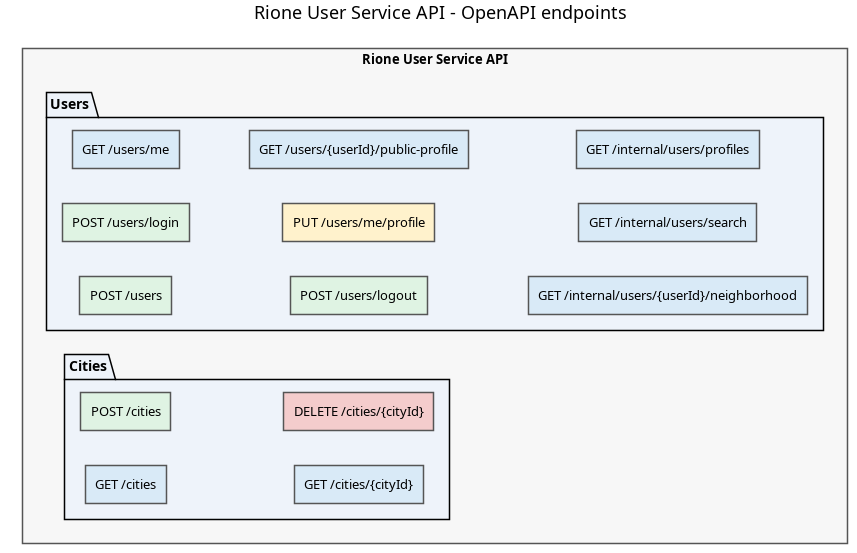
\includegraphics[width=0.95\textwidth]{generated/user-service_api.png}
    \caption{User Service OpenAPI diagram.}
    \label{fig:user-service-openapi}
\end{figure}

\begin{figure}[htbp]
    \centering
    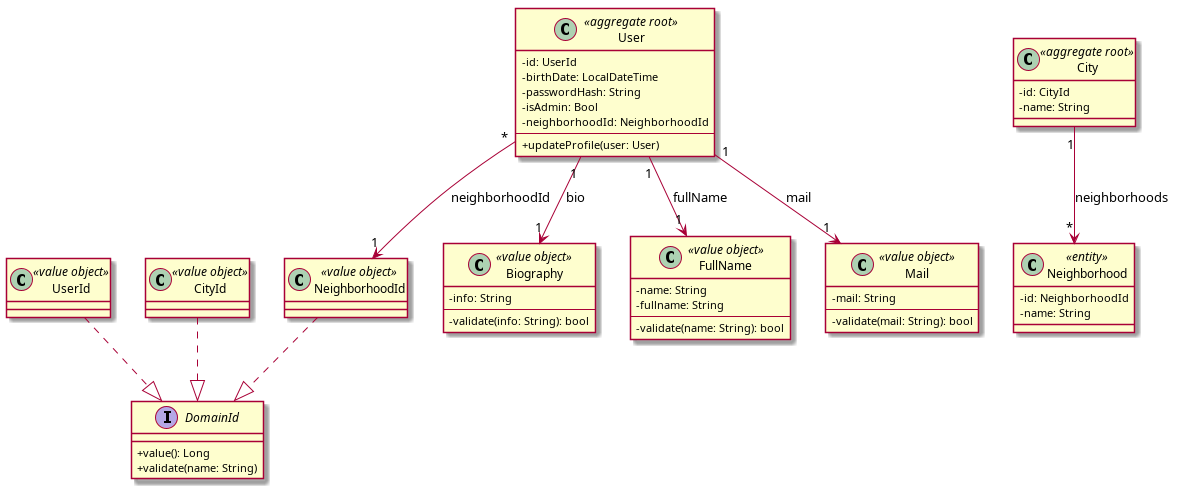
\includegraphics[width=0.95\textwidth]{generated/user_service.png}
    \caption{User Service domain model.}
    \label{fig:user-service-domain}
\end{figure}

\begin{figure}[htbp]
    \centering
    \includegraphics[width=0.95\textwidth]{\detokenize{user_c&c.png}}
    \caption{User Service component-and-connector diagram.}
    \label{fig:user-service-cc}
\end{figure}

\FloatBarrier

\subsection{Social Service}

The Social Service manages relationships between users inside the local social network. It is separated from the User Service because a user's profile and a user's social relationships follow different rules and lifecycles. Its domain model focuses on neighbour requests, neighborships, and blocks. It references users by identifier and uses proxy clients when it needs additional user data from the User Service. This keeps the relationship model independent while still allowing the service to enforce same-neighbourhood and blocking rules. Its API contract is shown in Figure~\ref{fig:social-service-openapi}, its domain model in Figure~\ref{fig:social-service-domain}, and its component-and-connector view in Figure~\ref{fig:social-service-cc}.

\begin{figure}[htbp]
    \centering
    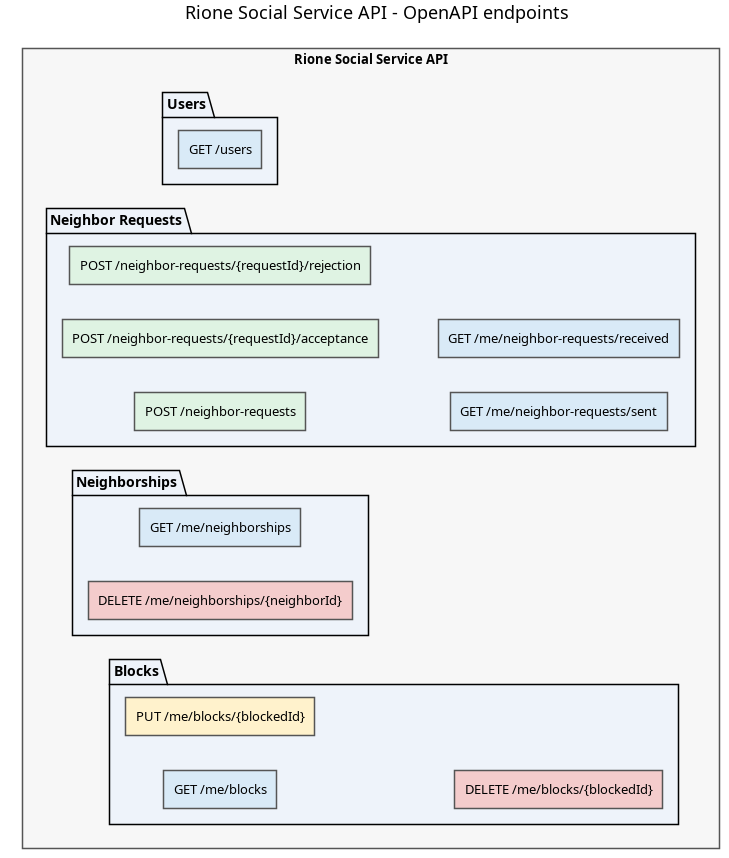
\includegraphics[width=0.95\textwidth]{generated/social-service_api.png}
    \caption{Social Service OpenAPI diagram.}
    \label{fig:social-service-openapi}
\end{figure}

\begin{figure}[htbp]
    \centering
    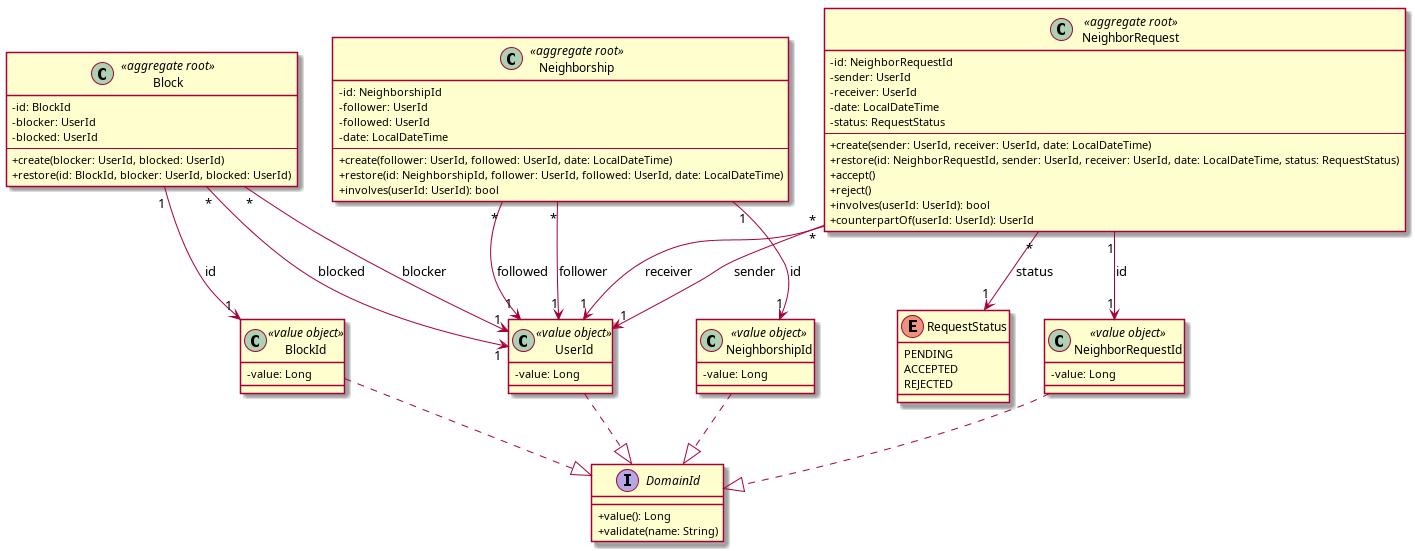
\includegraphics[width=0.95\textwidth]{generated/social_service.png}
    \caption{Social Service domain model.}
    \label{fig:social-service-domain}
\end{figure}

\begin{figure}[htbp]
    \centering
    \includegraphics[width=0.95\textwidth]{\detokenize{social_c&c.png}}
    \caption{Social Service component-and-connector diagram.}
    \label{fig:social-service-cc}
\end{figure}

\FloatBarrier

\subsection{Post Service}

The Post Service manages posts, comments, and reactions. It is the most write-intensive part of the system, so its model focuses on preserving content rules and interaction history. The Post aggregate owns the consistency boundary for content interactions, while comments and reactions are modeled as entities inside the aggregate. The service also publishes events when relevant interactions occur, allowing the Notification Service to react asynchronously through Kafka. Its API contract is shown in Figure~\ref{fig:post-service-openapi}, its domain model in Figure~\ref{fig:post-service-domain}, and its component-and-connector view in Figure~\ref{fig:post-service-cc}.

This service implements event sourcing for post state because posts can change through several user actions and the history of those actions is meaningful. Instead of storing only the latest snapshot of a post, the service stores an ordered stream of immutable events such as \texttt{PostCreated}, \texttt{PostContentUpdated}, \texttt{PostDeleted}, \texttt{CommentAdded}, \texttt{CommentUpdated}, \texttt{CommentRemoved}, \texttt{ReactionAdded}, \texttt{ReactionUpdated}, and \texttt{ReactionRemoved}. The current state of a post is rebuilt by reading the stream and applying each event in order. This makes the history of changes explicit and allows the service to derive the current post, comments, reactions, score, timestamps, and deleted state from the event sequence.

The event-sourcing boundary is exposed through the \texttt{PostEventStore} output port. The application service loads events with \texttt{read(postId)} or \texttt{readAll()}, reconstructs an in-memory \texttt{PostState}, validates the requested operation against that state, and appends one or more new events. The JPA adapter persists events in the \texttt{post\_events} table with a \texttt{postId}, an increasing \texttt{version}, an event \texttt{type}, an \texttt{occurredAt} timestamp, and a serialized payload. Appends use an expected version check; if the stored stream version differs from the expected one, the operation fails with a concurrency error. This gives the Post aggregate optimistic concurrency protection without exposing persistence details to the application core.

Event-sourcing events are kept separate from integration events. The internal post event stream is used to rebuild local state and compute metrics, while notification messages are published separately through the messaging adapter when comments or reactions should notify another user. Replaying the post event stream therefore reconstructs state without triggering external side effects.

\begin{figure}[htbp]
    \centering
    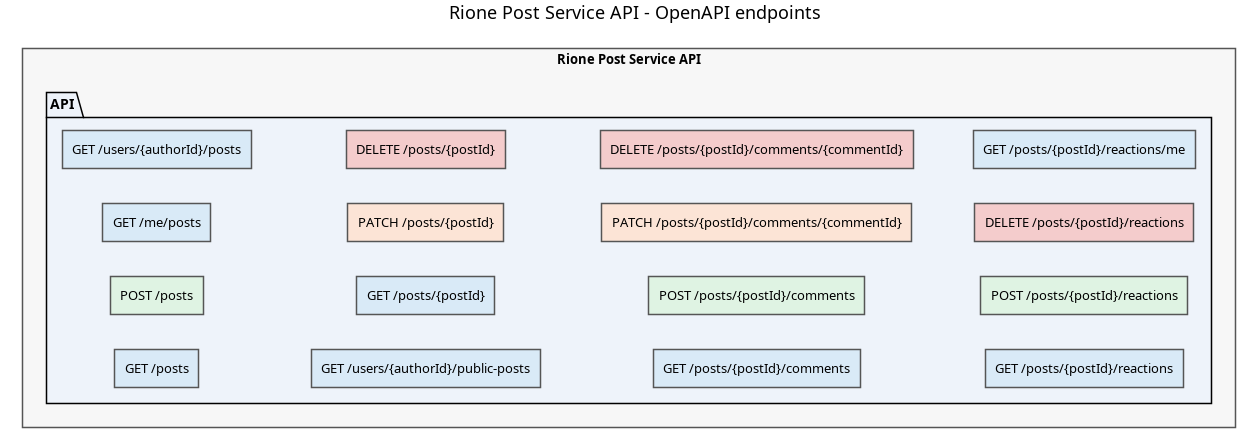
\includegraphics[width=0.95\textwidth]{generated/post-service_api.png}
    \caption{Post Service OpenAPI diagram.}
    \label{fig:post-service-openapi}
\end{figure}

\begin{figure}[htbp]
    \centering
    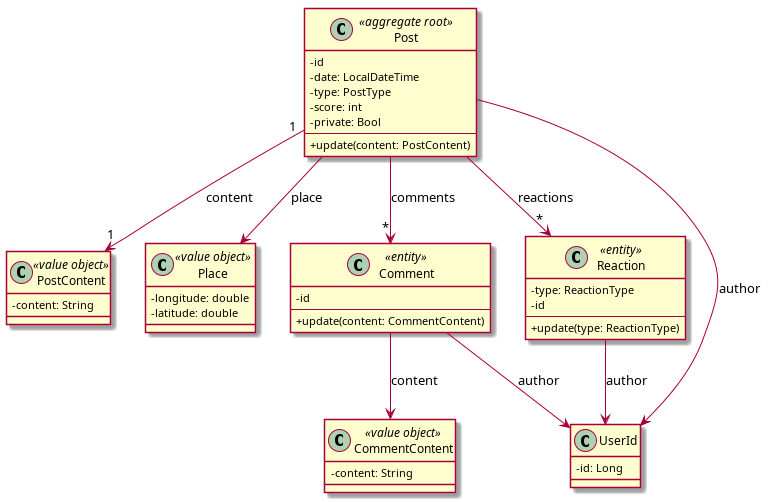
\includegraphics[width=0.85\textwidth]{generated/post_service.png}
    \caption{Post Service domain model.}
    \label{fig:post-service-domain}
\end{figure}

\begin{figure}[htbp]
    \centering
    \includegraphics[width=0.95\textwidth]{\detokenize{post_c&c.png}}
    \caption{Post Service component-and-connector diagram.}
    \label{fig:post-service-cc}
\end{figure}

\FloatBarrier

\subsection{Notification Service}
\label{sec:notification-service}

The Notification Service manages user notifications. It is separated from the workflows that generate notifications so that social and post actions can complete even if notification processing is delayed. Its domain model centers on the Notification aggregate, which records the recipient, actor, notification type, message, occurrence time, and read state. The service consumes Kafka events produced by other services and exposes read-side REST endpoints for retrieving and marking notifications as read. Its API contract is shown in Figure~\ref{fig:notification-service-openapi}, its domain model in Figure~\ref{fig:notification-service-domain}, and its component-and-connector view in Figure~\ref{fig:notification-service-cc}.

\begin{figure}[htbp]
    \centering
    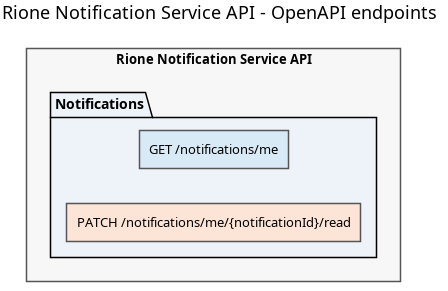
\includegraphics[width=0.85\textwidth]{generated/notification-service_api.png}
    \caption{Notification Service OpenAPI diagram.}
    \label{fig:notification-service-openapi}
\end{figure}

\begin{figure}[htbp]
    \centering
    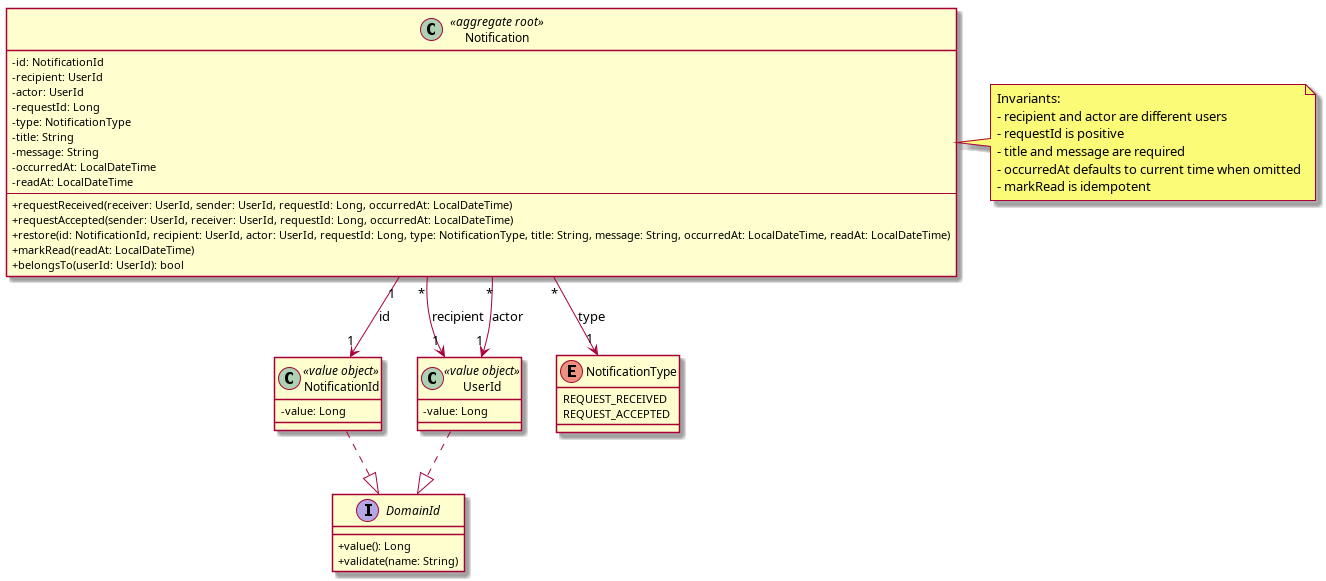
\includegraphics[width=0.95\textwidth]{generated/notification_service.png}
    \caption{Notification Service domain model.}
    \label{fig:notification-service-domain}
\end{figure}

\begin{figure}[htbp]
    \centering
    \includegraphics[width=0.95\textwidth]{\detokenize{notification_c&c.png}}
    \caption{Notification Service component-and-connector diagram.}
    \label{fig:notification-service-cc}
\end{figure}

\FloatBarrier

% =========================
% 8. Additional Patterns and Monitoring
% =========================
\section{Additional Patterns and Monitoring}

In addition to the core microservice, DDD, and hexagonal architecture choices, the project includes operational patterns that make the system easier to run and observe. These patterns do not implement business behavior directly, but they are necessary in a distributed system because failures are no longer limited to one process. A service can be alive but slow, a dependency can fail, or a business workflow can produce unusual activity. For this reason, the project uses health checks, circuit breakers, and application metrics together.

\subsection{Health API}

Each backend service exposes health information through Spring Actuator. This was used because Docker Compose and monitoring tools need a simple way to check whether a service is running and ready to receive traffic. The health endpoint is made available without user authentication, so operational checks do not need a normal user token. This is especially useful in a microservices architecture, where a failure may affect only one service while the rest of the system continues to run.

The health API is intentionally separated from the business OpenAPI contracts. Business APIs describe domain capabilities such as users, posts, social relationships, and notifications, while Actuator endpoints describe operational state. In the services, health and Prometheus endpoints are explicitly allowed by the security configuration. This keeps monitoring independent from business authentication while still protecting normal application operations.

Exposing the health endpoint is only useful if something polls it and reacts to a negative result, so the deployment layer was extended with a periodic liveness check and an automatic recovery action. Each backend container (API Gateway, User, Social, Post, and Notification services) now declares a Docker Compose \texttt{healthcheck} that calls \texttt{/actuator/health} every 15 seconds, with a 30-second startup grace period so the JVM boot time is not mistaken for a failure. This closes a gap that existed before: the \texttt{restart: unless-stopped} policy already present on every service only restarts a container when its process exits, so a service that is technically still running but reports \texttt{DOWN} (for example because it lost its database connection) would previously stay up and keep receiving traffic without any corrective action.

Docker itself only records a container as \texttt{unhealthy} in these cases; by default it does not take any further action. To close the loop, an \texttt{autoheal} sidecar container (\texttt{willfarrell/autoheal}) was added to \texttt{docker-compose.yml}. It watches the Docker socket, polls the health status of every container labeled \texttt{autoheal=true} (the five backend services above), and issues a \texttt{docker restart} as soon as a container is reported unhealthy. This gives the local deployment a simple, self-contained failure-recovery mechanism without introducing an orchestrator such as Swarm or Kubernetes, which would be disproportionate for a Docker-Compose-based, single-host setup. The API Gateway's and Social Service's \texttt{depends\_on} entries were also tightened to \texttt{condition: service\_healthy} on their upstream dependencies, so that dependent services only start routing traffic once the services they call are actually ready, not merely started.

\subsection{Circuit Breaker}

The project also uses the Circuit Breaker pattern to limit cascading failures during synchronous service calls. This pattern was added because the API Gateway depends on downstream services: if one of them becomes slow or unavailable, the gateway should not continue sending unlimited requests to it. The API Gateway applies circuit breakers to the routes that forward traffic to the User, Social, Post, and Notification services. When a downstream service becomes slow or repeatedly fails, the circuit can open and stop sending new calls for a short period, giving the failing service time to recover and preventing request queues from growing across the system.

Circuit breakers are configured through Resilience4j with count-based sliding windows, failure-rate thresholds, slow-call thresholds, and half-open recovery attempts. Their state is also exposed through Actuator health and circuit-breaker endpoints, so operational tools can observe whether a service dependency is closed, open, or recovering. This pattern complements health checks and metrics: health checks say whether a component is alive, metrics show runtime behavior over time, and circuit breakers actively protect callers from unstable dependencies.

\subsection{Application Metrics}

Application metrics are collected with Micrometer and exposed in Prometheus format through Spring Actuator. This was used because health checks only show a point-in-time status, while metrics show how the system behaves over time. The services expose \texttt{/actuator/prometheus}, and each service adds the \texttt{application} tag to its metrics so that Prometheus and Grafana can distinguish data coming from the API Gateway, User Service, Social Service, Post Service, and Notification Service.

The project includes both technical and business-oriented metrics. Technical metrics are provided by Spring Boot and JVM instrumentation and help observe runtime behavior such as HTTP requests, memory usage, CPU usage, and service availability. Business metrics are added where they provide useful insight into the application domain. For example, the User Service exports gauges for registered users, new users created today, and active users in the last five minutes. The Post Service exports gauges derived from the event store, such as total posts, posts created today, comments created today, and reactions created today.

Prometheus is responsible for scraping these metrics from the services, while Grafana is used to visualize them in dashboards. Example Grafana dashboard views are shown in Figure~\ref{fig:grafana-dashboard-overview} and Figure~\ref{fig:grafana-dashboard-details}. This combination makes it possible to monitor both infrastructure-level behavior and product-level activity. In practice, this helps detect service failures, observe user growth, and understand whether local community interaction is increasing through posts, comments, and reactions.

\begin{figure}[htbp]
    \centering
    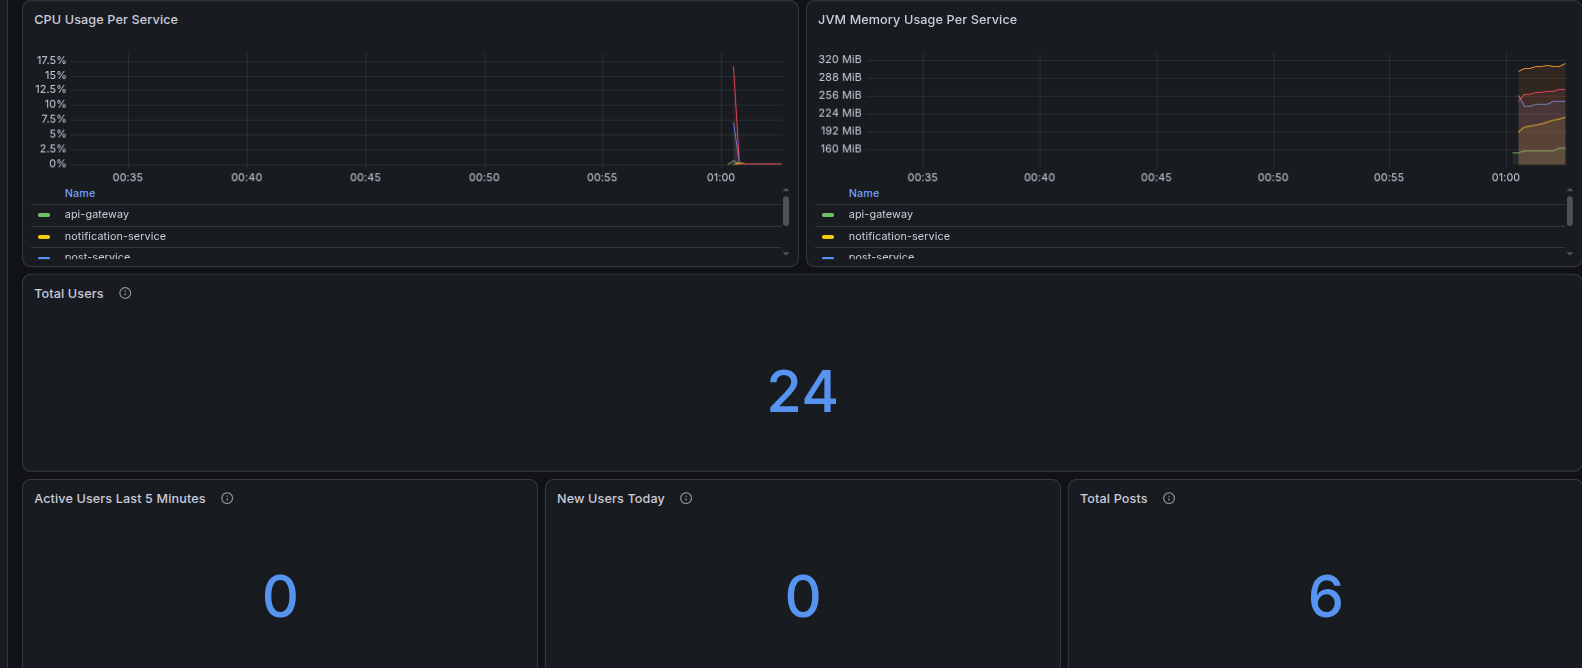
\includegraphics[width=0.95\textwidth]{dashboard/dash1.png}
    \caption{Grafana dashboard example for service and application metrics.}
    \label{fig:grafana-dashboard-overview}
\end{figure}

\begin{figure}[htbp]
    \centering
    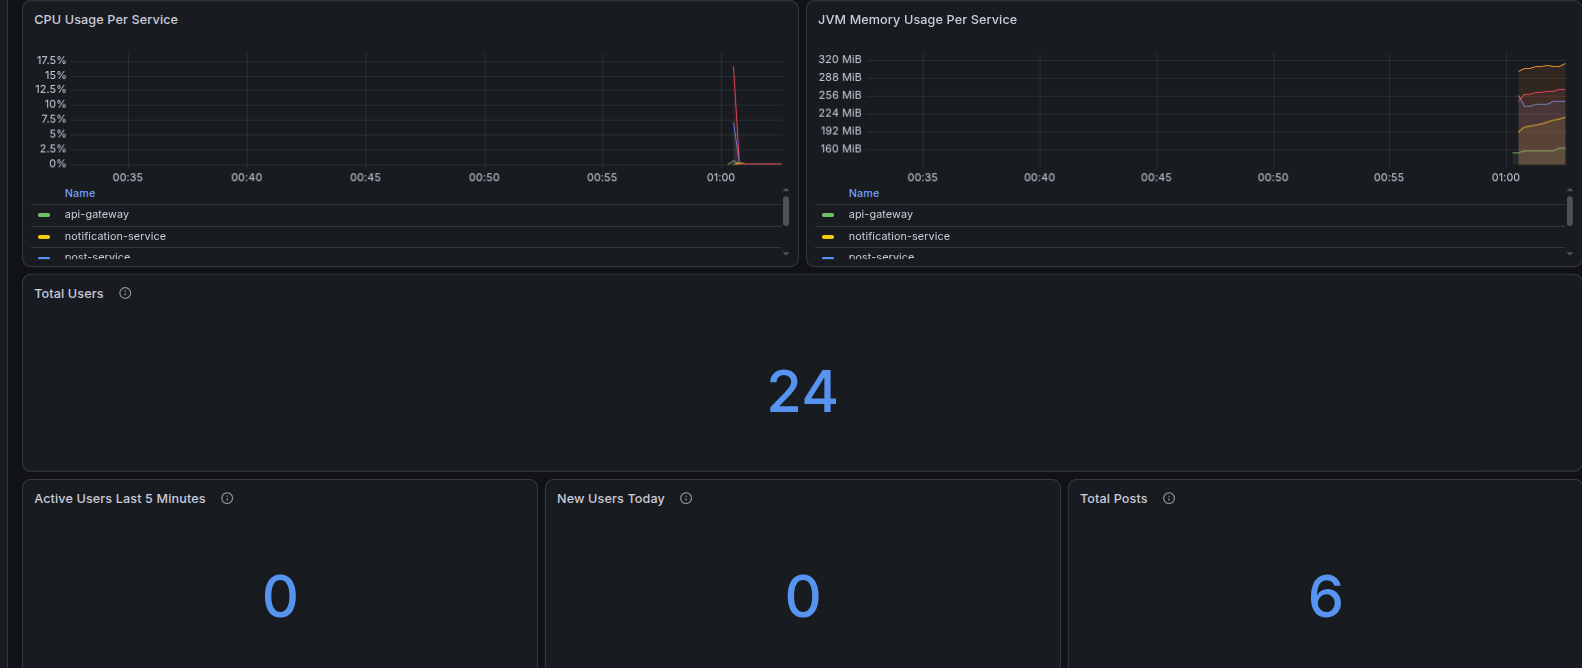
\includegraphics[width=0.95\textwidth]{dashboard/dash2.png}
    \caption{Grafana dashboard example with additional runtime metric panels.}
    \label{fig:grafana-dashboard-details}
\end{figure}

\FloatBarrier

\subsection{Service Level Objectives and Indicators}

Raw metrics show how the system behaves, but they do not by themselves say whether that behavior is acceptable. To close that gap, the project defines two Service Level Objectives (SLOs), each backed by a Service Level Indicator (SLI) that is actually measured rather than only described on paper.

The first SLO concerns the API Gateway, the single public entry point for every client request: 99.5\% of the requests it handles over a rolling window must return a non-5xx response. The corresponding SLI is the ratio of non-5xx to total responses, computed directly from the \texttt{http\_server\_requests\_seconds\_count} metric that Spring Boot Actuator and Micrometer already expose:

\begin{footnotesize}
\begin{verbatim}
sum(rate(http_server_requests_seconds_count{
    job="api-gateway", status!~"5.."}[$__rate_interval]))
/
sum(rate(http_server_requests_seconds_count{
    job="api-gateway"}[$__rate_interval]))
\end{verbatim}
\end{footnotesize}

No new instrumentation was required for this SLI, since the underlying metric was already collected as part of the technical metrics described above.

The second SLO targets the asynchronous flow between the Social Service and the Notification Service: when a user sends or accepts a neighbor request, the Social Service publishes a \texttt{REQUEST\_RECEIVED} or \texttt{REQUEST\_ACCEPTED} event to Kafka, and the Notification Service consumes it and persists a notification (see Section~\ref{sec:notification-service} and the event flow documented in \path{docs/events.md}). A notification that arrives too late undermines the purpose of the feature, so the SLO states that 95\% of these events must be consumed and turned into a notification within 2 seconds of publication. Measuring this SLI required extending the implementation: the Kafka listener in the Notification Service now records a Micrometer \texttt{Timer} for every event it consumes, using Micrometer's \texttt{serviceLevelObjectives(Duration.ofSeconds(2))} API so that the 2-second threshold is exposed directly as a Prometheus histogram bucket. The SLI is then:

\begin{footnotesize}
\begin{verbatim}
sum(rate(rione_social_event_delivery_seconds_bucket{
    le="2.0", job="notification-service"}[$__rate_interval]))
/
sum(rate(rione_social_event_delivery_seconds_count{
    job="notification-service"}[$__rate_interval]))
\end{verbatim}
\end{footnotesize}

Both indicators are visualized as dedicated panels on the same Grafana dashboard used for the other application metrics, with a red/green threshold at the SLO target, as shown in Figure~\ref{fig:grafana-slo-panels}. The full definitions, rationale, and query reference are kept in \path{docs/design/slo_sli.md}.

\begin{figure}[htbp]
    \centering
    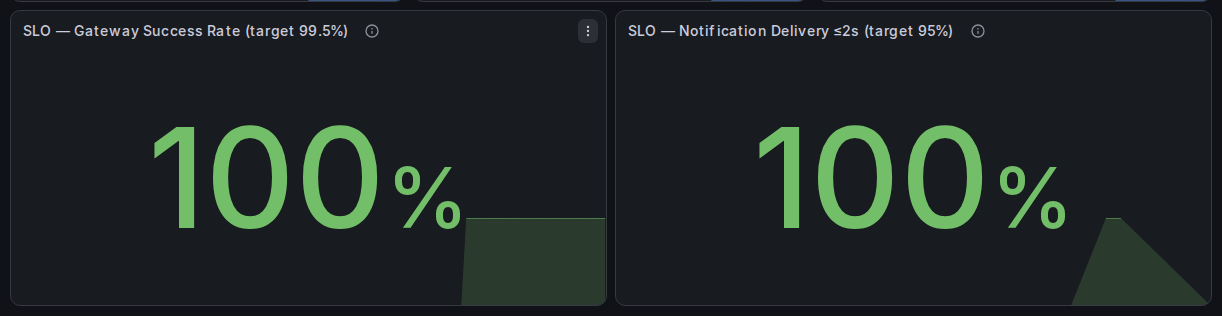
\includegraphics[width=0.95\textwidth]{dashboard/slo-panels.png}
    \caption{Grafana panels for the two SLOs: API Gateway success rate and notification delivery latency, both measured live against their targets.}
    \label{fig:grafana-slo-panels}
\end{figure}

\FloatBarrier

% =========================
% 9. Frontend
% =========================
\section{Frontend}

A lightweight frontend was implemented with React and Vite to make manual end-to-end testing easier. React was sufficient for this purpose because the frontend did not need complex server-side rendering or a production deployment pipeline; it needed a fast local interface that could call the backend and expose real workflows. Vite was used for the local development server because it starts quickly and works well for this kind of small client application.

The frontend interacts with the system only through the API Gateway, so it exercises the same public HTTP boundary used by external clients. This made it possible to verify authentication, profile management, neighbour search, neighbour requests, feed browsing, post reactions, comments, notifications, and administrative location management from a single user interface instead of testing each endpoint only through Swagger or direct HTTP calls.

The interface was intentionally kept simple and functional. Its purpose is not to replace backend tests, but to provide a practical way to validate complete user workflows across multiple services. For example, searching visible neighbours and sending requests can be tested from the view shown in Figure~\ref{fig:frontend-neighbor-search}; sent and received requests can be inspected from the neighbour management view shown in Figure~\ref{fig:frontend-neighbor-requests}; and post browsing, reactions, and comments can be tested from the feed shown in Figure~\ref{fig:frontend-feed}.

\begin{figure}[htbp]
    \centering
    
\includegraphics[width=0.95\textwidth]{\detokenize{ui/Screenshot from 2026-07-09 01-22-39.png}}
    \caption{React frontend view for searching visible neighbours and sending neighbour requests.}
    \label{fig:frontend-neighbor-search}
\end{figure}

\begin{figure}[htbp]
    \centering
    
\includegraphics[width=0.95\textwidth]{\detokenize{ui/Screenshot from 2026-07-09 01-22-55.png}}
    \caption{React frontend view for managing neighbours and pending requests.}
    \label{fig:frontend-neighbor-requests}
\end{figure}

\begin{figure}[htbp]
    \centering
    
\includegraphics[width=0.95\textwidth]{\detokenize{ui/Screenshot from 2026-07-09 01-24-05.png}}
    \caption{React frontend feed view for posts, reactions, and comments.}
    \label{fig:frontend-feed}
\end{figure}

\FloatBarrier

% =========================
% 10. Implementation
% =========================
\section{Implementation}

The implementation phase translated the previously defined requirements and architectural models into the running system. The main development effort focused on the backend microservices, their domain models, application use cases, REST and persistence adapters, integration mechanisms, observability support, and Docker Compose deployment.

Implementation was not treated as an isolated coding activity. The code was derived from requirements written before implementation and from manually designed UML diagrams, including domain models for the bounded contexts and component-and-connector diagrams for the overall architecture. This made the implementation phase closer to a controlled realization of the design than to an exploratory generation of services from vague prompts.

\subsection{Use of AI During Coding}

AI was used as a support tool during code generation, especially through agentic AI workflows. It was not used as a replacement for requirements analysis or architectural design. The project first defined requirements, bounded contexts, domain models, APIs, and component-and-connector diagrams manually. AI was then used to accelerate implementation inside those boundaries.

This distinction is important. A vague prompt such as ``create the Social Service'' would leave too many architectural and domain decisions to the tool. In this project, prompts were written after the design work, so the agent received concrete inputs and constraints. Typical backend prompts were closer to the following examples:

\begin{itemize}
    \item Given the requirements in \path{docs/requirements/social/} and the UML domain model in \path{docs/design/social_service.puml}, implement a missing validation rule in a Social Service value object. Keep validation inside the value object and preserve the existing DDD and Hexagonal Architecture structure.

    \item Given the component-and-connector diagram in \path{docs/design/social_c&c.puml}, fix the REST adapter so that it correctly maps application-layer exceptions to HTTP status codes without introducing domain logic into the controller.

    \item Given the requirements in \path{docs/requirements/post/} and the Post Service domain model in \path{docs/design/post_service.puml}, add support for a new domain event in the post aggregate, ensuring it is persisted through the existing \texttt{PostEventStore} port while keeping persistence events and integration events separated.
\end{itemize}

To make this use more controlled, custom AI skills were defined for the most relevant topics of the project, including Domain-Driven Design, Hexagonal Architecture, REST API design, Spring Boot testing, event sourcing, security, and related design principles. These skills were based on notes taken during the course and, where useful, on notes from technical books. Their purpose was to give the agent explicit project-specific guidance, so generated code would respect the architectural rules, package boundaries, testing expectations, and design vocabulary adopted in the project.

For the backend, the developer kept direct responsibility for requirements analysis, architectural design, testing strategy, debugging, and final validation. AI assisted with implementation details, repetitive code, test scaffolding, and refactoring suggestions, but its output was reviewed, adapted, and corrected against the intended design. In this sense, part of the coding activity was delegated to AI, while the most important engineering decisions remained developer-driven.

The frontend was the part most extensively delegated to AI. It was generated starting from visual mockups provided as prompts and then adapted to interact with the API Gateway and exercise the main application workflows. This was acceptable because the frontend was mainly intended as a lightweight testing and demonstration client, while the core architectural and domain complexity remained in the backend services.

% =========================
% 11. Conclusions
% =========================
\section{Conclusions}

The project analysis led to a decomposition that is coherent with both the domain and the expected runtime structure. Starting from the neighbourhood-based social network domain, the system was divided into User, Social, Post, and Notification bounded contexts. This separation made the model easier to reason about because each service owns a focused part of the ubiquitous language and can enforce its own business rules without sharing persistence models or internal domain objects with the others.

From a scalability point of view, this decomposition supports growth along several dimensions. A larger number of users can be handled by scaling the services that receive the most traffic, while the neighbourhood boundary keeps many social interactions local and reduces the need for global coordination. Growth in posts, comments, reactions, and notifications is also handled by separating write-heavy content workflows from notification delivery. Kafka allows notification processing to happen asynchronously, so services that produce events do not need to wait for every notification side effect to complete.

The database-per-service choice also supports scalability because each service can evolve its schema and persistence strategy independently. The Post Service is the most data-intensive component, and event sourcing makes its history explicit while preserving a reliable reconstruction path for current state. At the same time, this choice introduces operational responsibilities: event streams can grow significantly, so future versions should consider snapshots, archival policies, read models, and careful monitoring of replay time.

The architecture also includes operational mechanisms that become important as the system grows. Health checks, Prometheus metrics, Grafana dashboards, and circuit breakers provide visibility and protection in a distributed environment. They help detect service failures, observe usage trends, and prevent synchronous dependencies from propagating failures across services.

The main limitation of the current version is that it is still oriented toward a local Docker Compose deployment rather than a production-grade distributed platform. Future improvements could include service discovery, centralized configuration, stronger deployment automation, horizontal scaling policies, outbox-based event publication, database migration governance, and more complete dashboard definitions. These additions would make the architecture more robust under larger traffic volumes while preserving the domain-driven and hexagonal structure established in the project.

\end{document}
